\documentclass[11pt,a4paper]{article}
\usepackage[margin=2.5cm]{geometry}
\usepackage{amsmath,amssymb,amsfonts}
\usepackage{graphicx}
\usepackage{xcolor}
\usepackage{booktabs}
\usepackage{siunitx}
\usepackage[numbers,sort&compress]{natbib}
\usepackage{hyperref}
\hypersetup{colorlinks=true,linkcolor=blue,citecolor=blue,urlcolor=blue}
\graphicspath{{figures/}}

\newcommand{\ket}[1]{\lvert #1\rangle}
\newcommand{\bra}[1]{\langle #1\rvert}
\newcommand{\tr}{\mathrm{Tr}}
\newcommand{\code}{[\![5,1,3]\!]}

\title{\textbf{Variational syndrome-conditioned recovery for quantum error
correction: from unsupervised learning to a superconducting quantum
processor}}

\author{Author One$^{1}$, Author Two$^{1}$ \& Author Three$^{1,*}$\\
\small $^{1}$Affiliation, City, Country\\
\small $^{*}$corresponding author: email@example.edu}
\date{\today}

\begin{document}
\maketitle

\begin{abstract}
\noindent
Quantum error correction protects logical information by measuring stabilizer
syndromes and applying a syndrome-conditioned recovery, yet practical
decoders are rigid Pauli lookups that are provably sub-optimal for non-Pauli
noise, while learned decoders remain purely classical objects that are never
executed on hardware. Here we introduce \emph{variational
syndrome-conditioned recovery} (VSCR), a trainable quantum instrument that
combines projective stabilizer measurement with a learned, continuous,
syndrome-conditioned unitary recovery generated by a classical hypernetwork
and trained end-to-end without any error labels. Initializing each branch at
the exact Pauli-decoder correction makes training start at optimal
lookup-decoder performance, and we prove (Pauli-mixture noise) and verify
numerically (all channels) that this point is an \emph{exact} stationary point of
the unsupervised objective---a \emph{saddle} wherever certified headroom exists
above it. We therefore pair the warm start with a separable per-syndrome
refinement that escapes the saddle and with a decoder floor that makes
$\bar F_{\rm warm}\ge\bar F^{\rm dec}$ hold by construction. On the $\code$
perfect code VSCR reproduces the optimal decoder exactly on depolarizing and
mixed noise, where a per-branch semidefinite program certifies the decoder to be
optimal over \emph{all} CPTP recoveries (headroom $\le10^{-15}$), and
\emph{exceeds} it on amplitude-damping and coherent control-error noise---by
$+1.6\times10^{-3}$ at $p=0.10$ and $+3.1\times10^{-3}$ at $\varepsilon=0.30$,
capturing $90\%$ and $99.9996\%$ of the certified non-Pauli headroom---while
keeping every syndrome branch individually healthy, a property cold-started
variational recovery lacks. Ablations isolate the essential ingredients: removing
the syndrome projection collapses learned recovery on stochastic noise, an
independent per-syndrome parameterization is statistically indistinguishable from
the shared hypernetwork at this code size, and the closed-form noise-adapted Petz
recovery channel---the strongest recent training-free CPTP competitor---is
included as a genuine recovery baseline rather than an oracle estimator bound.
The trained instrument compiles to
fixed gate-level branch circuits that we verify against a density-matrix
simulator to $<10^{-9}$, and we design a Pauli-frame benchmark protocol that
reproduces the depolarizing channel exactly on hardware. We demonstrate the
protocol on the OriginQ Wukong 180-qubit superconducting processor: a
syndrome-conditioned recovery branch achieves post-selected logical fidelity
$0.80$ ($95\%$ Wilson interval $[0.68,0.88]$) against an ideal reference of
$1.000$, and we characterize the dominant hardware systematics---dysfunctional
mid-circuit measurement and ancilla-relaxation satellites. Our results
establish learned, hardware-executable recovery circuits as a practical
route to quantum error correction: label-free training starts at the optimal
Pauli decoder, provably never falls below it, saturates the optimal-CPTP recovery
ceiling wherever that ceiling coincides with the decoder, and exceeds the decoder
wherever it does not---all while remaining compilable to fixed gate-level branch
circuits.
\end{abstract}

\section*{Introduction}

Fault-tolerant quantum computation requires that logical information survive the noise of physical devices, and quantum error correction (QEC) is the
mechanism that makes this possible in principle~\cite{shor_code,steane_code,
knill_theory}. The last five years have turned this principle into an
experimental programme: surface-code logical qubits~\cite{fowler_surface,
google_scaling} whose error rates fall as
the code grows, logical error rates pushed below the surface-code
threshold~\cite{google_below_threshold}, logical operations in
error-detecting surface codes~\cite{marques_d3} and exponential error
suppression with cyclic bosonic codes~\cite{google_cyclic}, low-overhead
fault-tolerant memories from bivariate-bicycle codes~\cite{bravyi_bb},
real-time bosonic error correction beyond break-even~\cite{sivak_breakeven,
brock_qudits}, fault-tolerant gate sets in trapped
ions~\cite{ryan_anderson_rt,postler_ft,honciuc_832} and in reconfigurable
neutral-atom arrays~\cite{bluvstein_atoms}, and utility demonstrations on
noisy intermediate-scale processors~\cite{ibm_utility}. Small, dense codes
remain an attractive testbed in this landscape: the $\code$ perfect
code~\cite{laflamme_5q,gottesman_hamming} corrects any single-qubit error with
the minimum possible number of physical qubits, and has been benchmarked from
the earliest NMR implementations~\cite{knill_bench5q,zhang_nmr5q} to modern
cloud-accessible superconducting devices.

Every QEC experiment contains a \emph{recovery}: a map from measured syndrome
to corrective action. Standard recoveries are rigid Pauli lookups---optimal
for independent Pauli noise, but provably sub-optimal whenever the physical
noise is non-Pauli, as amplitude damping, crosstalk and coherent errors
are~\cite{knill_theory,beny_optimal,petz_map}. Approximate-QEC theory shows
that optimal recovery channels are generally non-unitary and
non-Pauli~\cite{petz_map,beny_optimal}, motivating recoveries that are
\emph{learned} rather than tabulated. Machine learning has so far entered QEC
almost exclusively through classical decoders---neural-network and
recurrent decoders for topological
codes~\cite{torlai_nn,baireuther_njp,meinerz_nn,wang_nn_boson},
high-accuracy learned decoders for superconducting
hardware~\cite{bausch_ml}, transformer architectures~\cite{tian_transformer}
and variational circuit compilers~\cite{xu_vcc}; on the quantum side,
variational encoders/recoveries such as QVECTOR~\cite{johnson_qvector}
optimize encoding and recovery circuits jointly for a device's noise.
Classical decoders improve the
classical processing step but never touch the quantum hardware: the
corrective operation applied to the qubits remains a Pauli frame update.
Complementarily, error-mitigation methods such as zero-noise
extrapolation~\cite{temme_zne,endo_zne,kandala_zne_hw}, virtual
distillation~\cite{huggins_vd,vikstal_vd} and Clifford data
regression~\cite{czarnik_cdr,cai_em_review} recover ideal expectation values
but require noise-scaling or multi-copy resources and provide no protected
logical subspace.

Here we close this gap with \emph{variational syndrome-conditioned recovery}
(VSCR): a variational quantum instrument in which a projective stabilizer
measurement is followed by a \emph{learned unitary} $R_s$, one per syndrome
branch, whose $60$ rotation angles are produced by a classical hypernetwork
and trained end-to-end, unsupervised, on the expected recovery fidelity.
Because each $R_s$ is an ordinary gate-level circuit, the trained instrument
is directly executable on quantum hardware---no classical decoder, no
real-time feedback, no Pauli-frame bookkeeping. Our contributions are:
(i)~a decoder-warm-started, label-free training scheme that begins exactly at
optimal Pauli-decoder performance and provably cannot start worse;
(ii)~a stationarity theorem and benchmarks showing that the optimal Pauli
decoder is an \emph{exact} critical point of the unsupervised branch-fidelity
loss---and a \emph{saddle} wherever certified headroom exists---together with a
separable per-syndrome refinement that provably cannot regress below the decoder
and that does capture that headroom. Warm-started VSCR thereby attains
decoder-optimal recovery on depolarizing and mixed noise, where a per-branch
semidefinite program shows the decoder to be CPTP-optimal (certified headroom
$\le10^{-15}$), and \emph{exceeds} the decoder on amplitude-damping and coherent
noise, where the headroom is $1.8\times10^{-3}$--$3.1\times10^{-3}$, while keeping
every syndrome branch individually healthy---in sharp contrast to cold-started
variational recovery. These claims are bracketed by same-family controls (an
independent per-syndrome variational recovery, a projection-free global
variational unitary), by the per-branch semidefinite-program ceiling, and by the
recent noise-adapted Petz recovery channel~\cite{biswas_petz} as a closed-form,
training-free CPTP competitor that is \emph{not} an oracle mitigation bound;
(iii)~an exact circuit-level compilation and
verification pipeline (worst circuit--simulator deviation $<10^{-9}$) together
with a Pauli-frame sampling protocol that emulates the depolarizing channel
exactly on hardware; and (iv)~a feasibility demonstration of the full protocol
on the OriginQ Wukong superconducting processor, including a quantitative
characterization of mid-circuit-measurement failure and ancilla-relaxation
systematics that any near-term QPU benchmark must confront.

\section*{Results}

\subsection*{A variational quantum instrument for syndrome-conditioned recovery}

We work with the $\code$ perfect code, whose stabilizer group
$S=\langle g_1,\dots,g_4\rangle$ with
$g_1=XZZXI$, $g_2=IXZZX$, $g_3=XIXZZ$, $g_4=ZXIXZ$ defines a
two-dimensional codespace spanned by $\ket{0_L},\ket{1_L}$ with logical
operators $X_L=XXXXX$, $Z_L=ZZZZZ$~\cite{laflamme_5q,gottesman_hamming}.
Distance three implies that the $16$ syndrome sectors
$P_s=\prod_i (I+(-1)^{s_i}g_i)/2$ (rank $2$ each) resolve all $15$
single-qubit Pauli errors uniquely. Physical noise is applied independently
to the five data qubits as (i)~depolarizing channels of rate $p$,
(ii)~amplitude-damping channels of rate $\gamma=p$, and (iii)~a mixed channel
(depolarizing $p$ followed by amplitude damping $p/2$).

VSCR replaces the Pauli lookup of a standard decoder by a learned unitary per
syndrome branch (Fig.~\ref{fig:schematic}a). Given a noisy logical state
$\rho$, the instrument applies the projective syndrome measurement and the
branch recovery, and its performance is the exact expectation over outcomes,
\begin{equation}
F(\phi)=\sum_{s=0}^{15}\bra{\psi}R_s(\phi_s)\,P_s\,\rho\,P_s\,
R_s^\dagger(\phi_s)\ket{\psi},
\label{eq:F}
\end{equation}
which is simultaneously the training objective (minimizing $1-F$) and the
reported recovery fidelity. Each $R_s$ is a hardware-friendly ansatz of three
layers of single-qubit $R_zR_xR_z$ rotations plus a ring of $R_{zz}$
entangling gates ($60$ parameters; Fig.~\ref{fig:schematic}b), so every
trained branch compiles to a fixed gate sequence. The $16$ angle vectors are
produced by a classical hypernetwork: a learnable syndrome embedding
$e_s\in\mathbb{R}^{24}$ passes through a $\tanh$ multilayer perceptron
($24\!\to\!64\!\to\!60$) yielding a correction $\Delta\phi_s$, and
\begin{equation}
\phi_s=\phi^{\rm dec}_s+\phi_0+\Delta\phi_s,
\label{eq:warm}
\end{equation}
where $\phi^{\rm dec}_s$ encodes the exact Pauli-decoder correction $C_s$ as
$\pi$-rotations ($X\!\to\!R_x(\pi)$, $Z\!\to\!R_z(\pi)$,
$Y\!\to\!R_z(\pi)R_x(\pi)$) and the hypernetwork output layer is
zero-initialised. Equation~\eqref{eq:warm} is the \emph{decoder warm start}:
at epoch zero $R_s=C_s$ exactly (verified to machine precision), so training
provably begins at optimal lookup-decoder performance and can only refine it
with continuous, non-Pauli corrections. Training is unsupervised: batches of
Haar-random logical states and sampled error rates feed
Eq.~\eqref{eq:F} directly through a fully differentiable density-matrix
simulator (complex128, Adam, curriculum in $p$); no error labels, no
syndrome--error pairs, and no classical decoder are used at any stage.
Model selection among seeds is likewise label-free, ranking candidates by the
worst per-branch conditional fidelity
$\mathrm{cf}_s=\mathbb{E}[\bra{\psi}R_sP_s\rho P_sR_s^\dagger\ket{\psi}]/
\mathbb{E}[\tr(P_s\rho)]$, which detects branches trapped in bad local
optima.

\subsection*{Unsupervised training reaches and refines decoder performance}

Figure~\ref{fig:training}a shows validation fidelity during training on the
depolarizing channel for three optimizers/initialisations. Genuine Adam
gradients through the differentiable simulator drive the warm-started model
to validation fidelity 0.9790, whereas the same architecture trained with
gradient-free random updates (the update rule of a broken reference
implementation) stalls near its initial value, confirming that the
improvement is attributable to real gradients. The warm start also removes
the principal failure mode of cold-started variational recovery: at
$p=0.15$ the worst-branch conditional fidelity is 0.812 for the warm
model versus 0.608 for an identically-architected cold-started model
and 0.812 for the Pauli decoder itself
(Fig.~\ref{fig:training}b), i.e.\ every syndrome branch of the trained
instrument is individually healthy, which is precisely the property a
hardware deployment requires.

\subsection*{Benchmarks: decoder-optimal where that is provable, better where it is not}

Figure~\ref{fig:benchmark} reports the average recovery fidelity
$\bar F(p)=\mathbb{E}_\psi[F]$ over $200$ Haar-random logical states per
point, together with the logical error rate $\Pr(F<0.9)$, for the three
incoherent noise channels (top and middle rows) and for a systematic coherent
control error (bottom panel). Two regimes appear, and they are exactly the two
regimes the ceiling analysis of the next subsection predicts.

\emph{Where the decoder is optimal, VSCR reproduces it exactly.} On depolarizing
and mixed noise the two agree to the last reported digit at every strength
($p=0.10$: depolarizing $0.946994568$ versus $0.946994568$; mixed $0.925338712$
versus $0.925338712$), while improving on the uncorrected state by a large margin
(raw $0.5908$ and $0.5229$). The agreement is structural rather than accidental:
the Pauli-decoder point $\phi_s=\phi^{\rm dec}_s$ is an \emph{exact} stationary
point of the Haar-averaged loss $1-F$ (gradient norms $\le6\times10^{-17}$ in
every channel tested; for Pauli-mixture noise this follows from a logical
two-design twirl, Methods), and the certified CPTP headroom above the decoder on
these two channels is $\le10^{-15}$---so there is nothing to gain and training
correctly stays put.

\emph{Where the decoder is sub-optimal, VSCR exceeds it.} On amplitude damping
the warm model reaches $\bar F=0.986349$ at $p=0.10$ against $0.984754$ for the
decoder ($+1.60\times10^{-3}$), and on the coherent channel the separation grows
monotonically with the over-rotation, from $2.5\times10^{-10}$ at
$\varepsilon=0.005$ to $+1.53\times10^{-3}$ at $\varepsilon=0.25$ and
$+3.09\times10^{-3}$ at $\varepsilon=0.30$ ($\bar F=0.99997$ versus $0.99688$).
These gains come from the separable per-syndrome refinement of Methods and
\emph{not} from gradient descent: the gradient stage on its own returns the
decoder to nine digits on both channels
($\bar F_{\rm grad}=\bar F_{\rm dec}=0.987894552$ over the amplitude-damping
curriculum and $0.999951843$ over the coherent one), because that point is a
saddle, and the refinement then captures $90.0\%$ and $99.9996\%$ of the
certified headroom respectively (ED Table~8). The resulting correction is genuinely
syndrome-dependent---after refinement the learned parts of the branch angle sets
differ by $\max_{s,s'}\lVert\Delta\phi_s-\Delta\phi_{s'}\rVert_\infty=9.3$
(amplitude damping) and $12.0$ (coherent), against $4\times10^{-16}$ on the
channels where the decoder is retained---so this is not a single global rotation
relabelled as a per-syndrome instrument. On every channel the decoder floor of
Methods guarantees $\bar F_{\rm warm}\ge\bar F^{\rm dec}$, and that guard is not
a formality: the gradient stage was measured to drift \emph{below} the decoder
($0.955524519$ versus $0.955524560$ on the depolarizing curriculum, $0.937977132$
versus $0.937977191$ on the mixed one), exactly the Adam-normalized random walk
that an identically vanishing gradient predicts. For context we include three
oracle error-mitigation upper bounds---Richardson zero-noise extrapolation
over exact noise-scaled states~\cite{temme_zne,endo_zne}, virtual
distillation~\cite{huggins_vd,vikstal_vd}, and a Clifford-data-regression-style
linear recovery over the full $1024$-component Pauli feature vector with
physical-state projection~\cite{czarnik_cdr,cai_em_review}. These methods
assume resources VSCR does not need (exact noise-scaled channels, multiple
copies, or complete single-shot tomography) and act on the full state without
any syndrome extraction or protected subspace; they delimit the
mitigation-oracle regime rather than serving as like-for-like competitors.
Projection lowers ZNE everywhere rather than raising it (depolarizing $p=0.10$:
$0.9104$ projected against $0.9570$ raw), which is the honest direction of the
correction---the raw estimator's apparent advantage was overshoot, not accuracy.

\emph{Petz recovery} is different in kind and is the comparison that carries
weight: a genuine recovery channel rather than an estimator, scored with the
identical fidelity functional. It is, however, handed the exact noise model, and
it is neither syndrome-resolved nor unitary. On the two Pauli-type channels it
falls clearly below both the decoder and VSCR ($0.9074$ versus $0.9470$
depolarizing, $0.8751$ versus $0.9253$ mixed, at $p=0.10$): one global channel
that does not condition on the syndrome cannot reverse branch-dependent damage.
On amplitude damping it leads ($0.9885$ versus $0.9863$), and on the coherent
channel it is exact---$\bar F=1.000000$ at every strength---because there the
noise \emph{is} a known unitary, which the Petz map inverts. Both facts are
informative rather than damaging. They bound what the projective,
syndrome-resolved, unitary family that VSCR occupies gives up, they identify
coherent over-rotation as the regime in which an explicitly noise-adapted
recovery is unbeatable, and they explain why our CPTP ceiling is a ceiling
\emph{given the projective readout} rather than an unconstrained one. What VSCR
alone provides is a \emph{label-free} recovery that needs no exact noise model and
compiles to a fixed gate-level branch circuit a processor can execute branch by
branch---the only method in Fig.~\ref{fig:benchmark} with that property.

\subsection*{Same-family baselines, ablations and an optimality ceiling}

The comparisons above pit VSCR against fixed decoders and oracle mitigation
methods; three additional controls compare it against \emph{learned}
recovery methods of the same variational-quantum family and establish how
close the achieved fidelity is to the information-theoretic optimum
(Fig.~\ref{fig:ablation}; ED Tables~5--9).
\emph{(i)~Independent per-syndrome recovery (no hypernetwork).} Replacing
the hypernetwork with a bare table of $16$ independent angle sets
($960$ parameters, no sharing; identical ansatz, loss, optimizer, curriculum,
decoder warm start \emph{and} identical separable refinement) changes nothing
material: the two architectures agree to within $2.3\times10^{-9}$ in $\bar F$
across the full $p$-grid on all four channels, and are bit-identical on
depolarizing and mixed noise (at $p=0.10$: depolarizing table $0.946995$ versus
hypernetwork $0.946995$; amplitude damping $0.986349$ versus $0.986349$). That
the refinement drives both to the same value is expected rather than
coincidental---it optimises the $16$ blocks independently and is therefore blind
to how the angles were parameterised---and it is the sharpest form of the point:
given identical post-processing, the shared hypernetwork buys no fidelity at this
code size. The refined table's worst-branch conditional fidelity also improves on
the decoder exactly where headroom exists ($0.633$ versus $0.538$ at amplitude
damping $p=0.15$) and matches it exactly where none does ($0.812$ versus $0.812$
depolarizing; $0.751$ versus $0.751$ mixed). In the cold-start low-data regime the independent table is if
anything stronger in the warm regime: trained on a fixed pool of $K$ logical
states and evaluated on fresh states, the two architectures are
\emph{indistinguishable} for every $K\in\{2,4,8,16\}$ ($\bar F=0.9470$,
$\min_s\mathrm{cf}_s=0.8717$), i.e.\ the decoder warm start alone reaches decoder
performance from as few as two training states. In the cold-start regime the
independent table does better at $K{=}4$ and $K{=}16$ ($\bar F=0.9470$,
$\min_s\mathrm{cf}_s=0.8717$) than the shared hypernetwork ($0.9060$--$0.9061$,
$\min_s\mathrm{cf}_s\approx0.39$), and the two tie at $K{=}2$; neither is monotone
in $K$, the expected behaviour of cold-started variational recovery in a
landscape whose decoder point is a saddle (ED Table~6). The hypernetwork is
therefore a deployment and scaling choice
at this code size---a table grows like $2^{n-k}$ while the hypernetwork
keeps fixed size and provides the exact per-branch decoder warm-start
construction---not a performance-critical component, and no claim of this
work relies on it.
\emph{(ii)~The projection is the load-bearing quantum ingredient.} A single
global variational unitary without syndrome measurement---the recovery half
of QVECTOR~\cite{johnson_qvector}, trained with the same ansatz and
budget---collapses on stochastic noise ($\bar F=0.5908,\ 0.7712,\ 0.5229$
at $p=0.10$ for depolarizing, amplitude damping and mixed noise, versus
$0.9470/0.9848/0.9253$ for the decoder and $0.9470/0.9863/0.9253$ for VSCR (the
middle entry being the refinement's gain); the depolarizing value matches
the raw-state fidelity within errors---the optimum of a unitary that cannot
reduce entropy): the measurement-based instrument, by contrast, purifies
every
branch. On the purely coherent channel the same global unitary inverts most
of the over-rotation ($\bar F=0.9962$ at $\varepsilon=0.10$), delimiting
the one regime in which a measurement-free variational recovery is
competitive.
\emph{(iii)~Ceiling over all CPTP recoveries.} For each branch we solved
exactly the semidefinite program for the optimal CPTP
recovery~\cite{reimpell_werner} (a $4\times4$ Choi program after reducing
the branch to the two-dimensional syndrome subspace; Methods). On the
Pauli-type channels the ceiling \emph{is} the decoder: its excess over
decoder fidelity is $\le4\times10^{-13}$ at $p\in\{0.05,0.10,0.15\}$
depolarizing and $+9\times10^{-7}$ for the mixed channel at $p=0.10$, so
under a projective syndrome readout \emph{no} recovery---learned or
hand-designed, unitary or general CPTP, Pauli or continuous---can beat the
values warm-started VSCR attains on these channels: it saturates the
ceiling rather than merely tracking a baseline. Small non-Pauli headroom
appears exactly where the noise is non-Pauli: $+1.8\times10^{-3}$ for
amplitude damping at $p=0.10$, and $+2.0\times10^{-4}$/$+3.1\times10^{-3}$
for coherent over-rotation at $\varepsilon=0.15/0.30$, where the ceiling
reaches exactly $1.0$ (a perfect recovery exists). The headroom is
concentrated in low-weight branches (e.g.\ conditional-fidelity headroom
$+0.20$ on a branch of weight $1.8\times10^{-3}$ for amplitude damping;
ED Table~7). Gradient descent from the warm start does not reach it, for the
structural reason set out in Methods: $\phi^{\rm dec}$ is an \emph{exact}
stationary point of the objective, so the headroom sits above a saddle that no
first-order method started there can leave. The separable per-syndrome
refinement does capture it---without labels and with no change to the
objective---reaching $90.0\%$ of the certified amplitude-damping headroom over
the training curriculum ($\bar F$ from $0.987894552$ to $0.989154346$ against a
ceiling of $0.989294324$) and $99.9996\%$ of the coherent one ($0.999951843$ to
$0.999999994$ against $0.999999995$), while on depolarizing and mixed noise,
where the certified headroom is exactly zero, it returns the decoder unchanged
and the floor prevents the drift below it that gradient training alone exhibits.
What remains genuinely out of reach is the \emph{discrete} part of the gap.
Consistently, restricting the learned recovery to Pauli
corrections collapses the unsupervised search to four logical classes per
branch: for depolarizing noise the exhaustive optimum reproduces the
perfect-code decoder table on every branch (cross-checked against
brute-force Pauli sampling to $2\times10^{-16}$), while for the coherent
channel ten low-weight branches prefer a different logical class (largest
conditional-fidelity gain $+0.68$ on a branch of weight $3\times10^{-5}$):
discrete moves invisible to local gradient descent but accounted for by the
ceiling. The decoder baseline is thus itself the optimal Pauli-restricted
learned recovery on Pauli-type noise, and VSCR generalizes it at zero cost
wherever Pauli corrections are already optimal.

\subsection*{Exact circuit compilation and a Pauli-frame hardware protocol}

To move the trained instrument onto hardware we compile each branch to a
fixed circuit (Fig.~\ref{fig:schematic}c): state preparation, a synthesized
Clifford encoder ($36$ gates, verified against the codespace isometry with
overlap $1-10^{-15}$), an injected Pauli frame, the stabilizer extraction
unitary (basis rotations plus CNOT parity ladders onto four ancillae), the
branch recovery $R_s(\phi_s)$ with each $R_{zz}$ decomposed as
CNOT--$R_z$--CNOT, the inverse encoder, and logical-basis readout. Because
the recovery is branch-fixed, no classical processing or feed-forward occurs
inside the circuit: post-selection on the ancilla register implements the
projector $P_s$ offline. Depolarizing noise is emulated \emph{exactly} by
sampling Pauli frames ($I$ with $1-p$, $X,Y,Z$ with $p/3$ per data qubit) and
averaging---the frame-randomization spirit of randomized
compiling~\cite{wallman_rc} applied to benchmark design---so frame statistics
reproduce the channel expectation of the density-matrix simulator without any
stochastic approximation; the estimated fidelity is
$F(p)=\mathbb{E}_{\rm frames}\sum_s P(s)F_s$ with
$F_s=P(\text{data}=00000\mid s)$.

We verify the compilation at the amplitude level with a dense $512$-dimensional
statevector simulation of every branch circuit, including the mid-circuit
ancilla projection: the worst deviation between circuit-level and
density-matrix fidelities over all frames, logical states and noise rates is
8.0\times 10^{-15}, i.e.\ the hardware protocol and the training simulator are the
same mathematical object. The same pipeline yields the exact ideal reference
for every branch ($16$ frames $\times$ $2$ logical states), tabulated in
Extended Data, against which hardware estimates are compared point by point.
A late-measurement variant, in which the four ancilla readouts are moved to
the end of the circuit, has an exactly identical joint distribution over
(ancilla, data) outcomes whenever no feed-forward is present; we use it on
hardware because, as shown below, mid-circuit measurement is dysfunctional on
the target processor.
\subsection*{Feasibility demonstration on the OriginQ Wukong processor}

We executed the protocol on the OriginQ Wukong superconducting processor
(chip \texttt{WK\_C180}, $180$ qubits) through the pyQPanda3 cloud
interface~\cite{pyqpanda3,originq_cloud}, using compiler options
(amendment, qubit mapping, optimization) and a fixed best-quality $9$-qubit
physical block; the returned bitstring layout was established empirically as
$[a_3a_2a_1a_0][d_4d_3d_2d_1d_0]$ by hypothesis scoring over data-hit
evidence. Four branch circuits ($400$ shots each) probe the two measurement
schemes and two error injections (Fig.~\ref{fig:hardware}).

Three findings define the operating envelope of near-term QPU QEC
benchmarks. First, \emph{mid-circuit measurement is dysfunctional} on this
device: for both mid-measure circuits the post-selected data register never
reproduces the decoded logical state ($0$ hits in $735$ shots across all
layout hypotheses), while the late-measure variants retain syndrome
correlation. Second, the error-injected branch shows genuine
syndrome-conditioned recovery: for an injected $X_2$ error (syndrome
$s=12$) the hardware syndrome distribution peaks at $s=12$ with a dominant
satellite at $s=8$---the signature of ancilla $a_1$ relaxing during the
late-measurement wait, occurring $1.75\times$ more often than the correct
peak---and, post-selecting on correctly read syndromes, the recovered logical
state is correct in $44/55$ shots, $F_{12}=0.80$ ($95\%$ Wilson interval
$[0.68,0.88]$) against an ideal reference of $1.000$. Third, the
identity branch ($s=0$, no injected error) is dominated by accumulated
gate and readout errors over the $\sim\!160$-gate circuit: the expected
bitstring appears in only $2.4\%$ of shots and the syndrome distribution is
nearly uniform, quantifying the distance between current cloud hardware and
the fault-tolerant regime for dense codes. The total-variation distances
between hardware and ideal joint distributions ($0.88$ for the injected
branch, $0.98$ for the identity branch) are consistent with these
observations and motivate readout-error mitigation and shorter extraction
schedules in the full benchmark, whose design ($2$ logical states $\times$
$2$ error rates $\times$ $2$ Pauli frames $\times$ $16$ branches at $10^3$
shots) and exact ideal reference are specified in Methods and Extended Data.

\section*{Discussion}

VSCR occupies a middle ground that previous work leaves empty: it keeps the
projection (purification) power of measurement-based decoding, like a
classical decoder, while making the corrective operation itself a trainable,
continuous quantum circuit, like approximate-QEC recovery
maps~\cite{petz_map,beny_optimal}. The decoder warm start
(Eq.~\ref{eq:warm}) is what makes this combination practical: variational
recovery trained from random initialization suffers bad per-branch local
optima (Fig.~\ref{fig:training}b), whereas starting from $C_s$ puts the
optimizer at a point whose value is already decoder-optimal. Our stationarity
result explains both the strength and the precise limit of that choice. The
decoder is an \emph{exact} critical point of the Haar-averaged branch-fidelity
loss on every channel we test---not a small-gradient region but a true zero,
which we verify by autograd ($8.3\times10^{-19}$) and by central finite
differences (exactly $0$)---so warm training inherits decoder optimality,
per-branch health and hardware compilability wherever the decoder is already
optimal, and, with the decoder floor of Methods, cannot drift below it
anywhere. But on channels where the decoder is \emph{sub}-optimal the same
stationarity makes it a saddle: the certified headroom above it is exactly the
eigenvalue gap $\lambda_{\max}(Q_s)-\lambda(G^{\rm dec}_s)$, and no first-order
method started there can cross it. That is a property of the loss landscape
rather than of the ansatz, which is why we add the separable per-syndrome
refinement: because the branch weight cancels in the objective, the sixteen
blocks are exactly independent and can be re-optimized individually from large
symmetry-broken starts, and that does reach the certified optimum. Regimes in
which learned corrections deviate from Pauli decoding even under plain gradient
training---logical-state-biased ensembles, hardware-measured
losses that break the logical twirl, or device-native correlated noise
entered directly into the training channel---are identified by the same
analysis and are the natural targets for hardware-in-the-loop training once
shot budgets allow.

The ablations sharpen what is and is not claimed. Within the
projective-readout protocol the Pauli decoder is the \emph{optimal} recovery
on the Pauli-type channels at every strength we tested (SDP ceiling over all
CPTP maps, ED Table~7), so the decoder-parity of warm-started VSCR there is
ceiling-saturation, not a missed opportunity; amplitude-damping and coherent
noise leave a small non-Pauli headroom ($1.8\times10^{-3}$ and up to
$3\times10^{-3}$, concentrated in low-weight branches). Local gradient descent
from the stationary decoder point cannot reach it---that point is a saddle, not a
minimum---but the separable per-syndrome refinement does, capturing $90.0\%$
(amplitude damping) and $99.9996\%$ (coherent) of the certified headroom, with
the decoder floor guaranteeing that no channel regresses. That is where the
boundary between certification and genuine learned improvement now lies: the
\emph{continuous} part of the headroom is captured, and only the \emph{discrete}
part---the Pauli-class moves tabulated in ED Table~7---remains out of reach of
any continuous method.
The projection---not the parameterization---is the essential quantum
ingredient: removing it collapses learned recovery on stochastic noise
(QVECTOR-style global unitary), while removing the hypernetwork (a
per-syndrome independent table) leaves warm-started performance unchanged at
$n=5$ and even dominates in the cold-start low-data regime; the shared
architecture is motivated by $2^{n-k}$ syndrome-space scaling, not by
accuracy at this code size.

The hardware part of this work is deliberately a feasibility study, and its
limitations are informative. Post-selection costs samples in proportion to
$P(s)$, and on \texttt{WK\_C180} ancilla relaxation during the late-measure
wait redistributes that weight toward lower-weight syndromes; both effects
are measurable and correctable in analysis (relaxation-aware branch
assignment, readout mitigation~\cite{vandenberg_readout}) but they consume
shots. Mid-circuit measurement---the standard route to feed-forward
recovery---is unavailable on this processor, which is why our protocol is
branch-fixed and feedback-free; platforms with fast mid-circuit
readout~\cite{sivak_breakeven,ryan_anderson_rt} could execute the same trained
branches with real-time selection. Extending VSCR to larger codes requires
only that the syndrome measurement remain projective: a per-syndrome
parameter table matches the hypernetwork at $n=5$ (ED Table~6) but grows
like $2^{n-k}$, whereas the hypernetwork keeps fixed size and shares
statistical strength across branches; branch circuits
remain fixed-depth, though shot budgets grow with the syndrome count.
Combining learned branch recoveries with classical decoders (VSCR refining
the residual error after a lookup step) and with error
mitigation~\cite{cai_em_review,suzuki_em} are natural next steps.

Taken together, our results show that a quantum error-correcting recovery can
be \emph{learned as a circuit}, certified optimal at the compiler level
without labels, and executed branch by branch on a cloud superconducting
processor---a route to error correction that complements the rigid Pauli
decoding used in today's large-scale experiments.
\section*{Methods}

\paragraph{Simulator and code.}
All training and evaluation use a fully differentiable density-matrix
simulator (PyTorch, complex128) over the $32$-dimensional physical space of
the $\code$ code. Stabilizers, the codespace projector, the $16$ syndrome
projectors $P_s$, and the logical basis ($\ket{0_L}$ the $+1$ eigenstate of
$Z_L$ in the codespace, $\ket{1_L}=X_L\ket{0_L}$) are constructed exactly and
asserted at import (codespace rank $2$, mutual commutation, isometry).
Noise channels are applied as exact Kraus maps per data qubit: depolarizing
of rate $p$, amplitude damping of rate $\gamma=p$, their mixture (depolarizing
$p$ then damping $p/2$), and a coherent control-error channel applying an
identical over-rotation $R_x(\varepsilon)$, $\varepsilon=p$, to every data
qubit.

\paragraph{VSCR architecture and training.}
$R_s$ comprises $3$ layers of $\{R_z,R_x,R_z\}$ on each of $5$ qubits plus a
ring of $R_{zz}(q,q{+}1\bmod 5)$, i.e.\ $60$ angles. The hypernetwork maps a
learnable embedding $e_s\in\mathbb{R}^{24}$ through Linear$(24,64)$--tanh--
Linear$(64,60)$ to $\Delta\phi_s$; a shared offset $\phi_0$ and a per-branch
residual $\phi^{\rm ex}_s$ are also carried, so that
$\phi_s=\phi^{\rm dec}_s+\phi_0+\Delta\phi_s+\phi^{\rm ex}_s$. Only the
\emph{output} layer is zero-initialised, which is precisely what makes
$\phi_s\equiv\phi^{\rm dec}_s$ at step $0$; the hidden layer keeps a
non-degenerate $\mathrm{std}=1/\sqrt{24}$ init and the embedding is drawn from a
private generator, so it is reproducible independently of the training seed.
This distinction is load-bearing rather than cosmetic. An all-zero tanh-MLP
passes no gradient to its own weights \emph{or} to its embedding---the hidden
activation is identically zero, so the output layer's gradient, which is
proportional to it, vanishes too---leaving $\phi_0$ as the only trainable part of
the syndrome pathway, i.e.\ a single global rotation shared by all sixteen
branches. A self-test asserts that every syndrome-pathway parameter moves under
the real label-free loss and that the sixteen branch angle sets become mutually
distinct, so this cannot silently regress.

Training minimizes $1-F$ (Eq.~\ref{eq:F}) with Adam in a three-stage curriculum
(low-$p$, full-range, low-rate polish; $1700$ epochs per seed), for seeds
$\{1234,2024\}$ per channel; selection uses the label-free worst-branch
conditional fidelity at $p=0.07$. Both the objective and the selection
diagnostic are evaluated by \emph{exact} deterministic quadrature rather than by
sampling. A $3$-node Gauss--Legendre rule in $\cos\theta$ times a $7$-point
equispaced azimuthal grid reproduces the Haar average of any degree-$2$ Bloch
polynomial to machine precision, and a $6$-node Gauss--Legendre rule averages the
noise strength over the curriculum interval. Because
$\bra{\psi}R_sP_s\rho P_sR_s^\dagger\ket{\psi}$ probes only the two-dimensional
syndrome subspace, the $60$-gate ansatz is applied to two columns instead of a
full $32\times32$ unitary, so the exact objective costs $1.5$\,ms per epoch
against $67$\,ms for the equivalent sampled loop ($47\times$). This matters
quantitatively rather than merely aesthetically: the non-Pauli headroom to be
resolved is $1.9\times10^{-4}$--$3.7\times10^{-3}$, whereas a $48$-sample
Monte-Carlo estimator has a standard error of $1.1\times10^{-4}$ at amplitude
damping $p=0.10$. The effect sits at the noise floor of the sampled estimator, so
only a zero-variance gradient can both resolve it and descend on it.

\paragraph{Escaping the decoder saddle: separable refinement and a decoder floor.}
Gradient training alone returns essentially the decoder, and the reason is
structural rather than a tuning failure. Each branch contribution is a $4\times4$
Rayleigh quotient $g_s^\dagger Q_s g_s$ with
$g_s=\mathrm{vec}(V^\dagger R_sW_s)$ and $\lVert g_s\rVert$ fixed, and the
gradient of a Rayleigh quotient vanishes \emph{exactly} at the eigenvectors of
$Q_s$. The decoder's $2\times2$ block is such an eigenvector on every branch of
every channel: at $\phi^{\rm dec}$ we measure
$\max_{s,k}\lvert\partial\bar F/\partial\phi_{s,k}\rvert=8.3\times10^{-19}$ by
autograd and exactly $0.0$ by central finite differences. Wherever
$\lambda(G^{\rm dec}_s)<\lambda_{\max}(Q_s)$ the decoder is therefore a
\emph{saddle}, and the certified headroom
$\bar F^{\rm unit}-\bar F^{\rm dec}$ is precisely that eigenvalue gap. No
first-order method started there can move off it, and small symmetry-breaking
offsets do not help either: measured capture is $-0.52\%$ to $-0.03\%$ for
$\epsilon\in[10^{-4},10^{-1}]$, because a random $60$-angle offset lies almost
entirely in the ansatz's null directions and Adam then random-walks on
round-off-level gradients.

What does work exploits an exact separability. Writing the Haar-averaged branch
fidelity as $\mathrm{cf}_s=(J_s+\mathrm{const}_s)/6/p_s$, the branch weight
\emph{cancels} in the objective, $p_s\,\mathrm{cf}_s=(J_s+\mathrm{const}_s)/6$,
so the $p$-averaged fidelity decomposes as
$\bar F_{\rm avg}=\sum_s \mathrm{obj}_s(\phi_s)$ with the sixteen blocks mutually
independent---even after the $p$-average, since reordering the two sums leaves
each block a function of $\phi_s$ alone. Optimizing the blocks separately
therefore reaches the global optimum of the per-syndrome-unitary family, with no
cross-branch coupling to coordinate. We do so from a few \emph{large}
symmetry-broken starts ($\mathcal{O}(1)$-radian offsets), always retaining the
incumbent as start $0$ and accepting a candidate only on strict improvement, so
the refinement is monotone by construction. A self-test asserts that this block
objective equals the production quadrature objective to $\sim10^{-16}$ for
\emph{arbitrary} angle tables (not merely code-preserving ones), that the refined
table stays code-preserving to $\sim10^{-5}$, and that the result never exceeds
the certified ceiling.

The candidates are then floored. Among
$\{\phi^{\rm dec},\phi^{\rm grad},\phi^{\rm refined}\}$ we keep whichever
maximizes the exact production objective, so
$\bar F_{\rm warm}\ge\bar F^{\rm dec}$ holds \emph{by construction} rather than
by hope. This guard is not vacuous: on channels whose certified headroom vanishes
the gradient stage drifts \emph{below} the decoder---exactly the
Adam-normalized random walk predicted by the zero gradient---and the floor is
what keeps that drift from becoming a reported regression.

\paragraph{Stationarity of the Pauli decoder.}
For a Pauli-mixture channel each branch state is a mixture
$\sum_E w_E E\ket{\psi}\bra{\psi}E^\dagger$ of unitarily rotated logical
states. The first-order variation of $\mathbb{E}_\psi[\bra{\psi}G M_\psi
\ket{\psi}]$ along an anti-Hermitian generator $G$ then reduces, via the
complex two-design moment
$\mathbb{E}[\bra{\psi}X\ket{\psi}\bra{\psi}Y\ket{\psi}]=(\tr X\,\tr Y+
\tr XY)/(d(d+1))$ on the two-dimensional logical space, to combinations of
$\tr(G')$ and $\tr(G'W)$ with $W$ a logical Pauli image of a traceless
Pauli-like operator; both vanish, so $\phi_s=\phi^{\rm dec}_s$ is a critical
point of the Haar-averaged loss. Numerically the same stationarity holds for
amplitude damping and for the coherent channels (gradient norms
$\le6\times10^{-17}$), which we attribute to the logical twirling induced by
the Haar ensemble; ensembles or losses that break this twirl (fixed logical
states, hardware-measured fidelities) admit non-vanishing gradients and hence
genuine learned deviations.

\paragraph{Baselines.}
\emph{Perfect-code decoder}: exact expectation of the optimal single-error
Pauli lookup $\sum_s\bra{\psi}C_sP_s\rho P_sC_s^\dagger\ket{\psi}$.
\emph{ZNE-phys (oracle)}: Richardson extrapolation over exact states at noise
scales $\{1,2,3\}$~\cite{temme_zne,endo_zne}, with the extrapolated operator
projected onto the nearest positive-semidefinite trace-one state before scoring.
The projection is not cosmetic. The raw estimator
$\bra{\psi}\big(3\rho(p)-3\rho(2p)+\rho(3p)\big)\ket{\psi}$ is an
\emph{unbounded} linear functional of the extrapolated operator: nothing in its
definition keeps that operator inside the state space, so nothing keeps $F\le1$.
On the coherent channel it does not, and pervasively: across a $60$-state audit
the raw estimator exceeds $1$ for \emph{every} state at \emph{every} noise
strength probed, from $1.00000002$ at $\varepsilon=0.005$ to $1.1306$ at
$\varepsilon=0.30$ ($1.0118$ at $\varepsilon=0.15$). On the three incoherent
channels it never exceeds $1$ ($0/60$ states at every strength), which is
precisely why the artefact went unnoticed---it is specific to the unitary
channel, where the extrapolated operator lies furthest from the state space. An
unprojected ZNE curve therefore ``wins'' the coherent panel purely by overshooting
physical fidelity, which is an estimator artefact and not a result. We therefore
report the projected estimator, cap every fidelity axis at exactly $1$ with the
physical ceiling drawn as a reference line, assert $F\le1+10^{-9}$ for every
method, and record the raw overshoot per noise strength as an audit
(ED Table~9), so that the artefact stays visible rather than being silently
removed.
\emph{VD (oracle)}: normalized $\rho^2$~\cite{huggins_vd}. On a purely coherent
channel $\rho$ is pure, so $\rho^2=\rho$ and the $k{=}2$ VD estimator is
algebraically identical to Raw; rather than draw a duplicate curve and imply a
comparison that does not exist, we assert the identity to machine precision and
omit VD from that panel. \emph{LinDR-phys (oracle)}: ridge regression from
noisy to ideal Pauli-feature vectors ($1024$ features, $1500$ training states,
ridge selected on validation) with the reconstruction projected onto the
nearest positive-semidefinite trace-one state before scoring, in the spirit of
Clifford data regression~\cite{czarnik_cdr}. These three are error
\emph{mitigation} estimators with oracle access (exact noise-scaled channels,
exact copies, full tomography) and are reported as upper bounds only.

\emph{Petz recovery (2024)}: the noise-adapted recovery map, i.e.\ the transpose
channel~\cite{petz_map,beny_optimal},
\begin{equation}
\mathcal{R}_{\sigma,\mathcal N}(X)=\sigma^{1/2}\,
\mathcal N^\dagger\!\Big(\mathcal N(\sigma)^{-1/2}\,X\,
\mathcal N(\sigma)^{-1/2}\Big)\,\sigma^{1/2},
\qquad \sigma=P_{\rm code}/2,
\label{eq:petz}
\end{equation}
with $\mathcal N$ the exact noise channel and $\mathcal N(\sigma)^{-1/2}$ taken on
the support of $\mathcal N(\sigma)$, in the form for which circuit constructions
were recently given and demonstrated on an amplitude-damping-adapted four-qubit
code by Biswas \emph{et al.}~\cite{biswas_petz}. This is the comparator that
actually carries weight. Unlike ZNE/VD/LinDR, Petz is a genuine recovery
\emph{channel}: closed-form, training-free, noise-adapted and CPTP, and
provably close to optimal among all CPTP recoveries whenever the
Knill--Laflamme conditions hold approximately---precisely the regime of a
distance-$3$ perfect code at these rates. It therefore sits in the same category
as the decoder and as VSCR, and it is scored with the \emph{identical} estimator
$\bra{\psi_{\rm enc}}\mathcal R(\rho_{\rm noisy})\ket{\psi_{\rm enc}}$, so the
comparison introduces no method-dependent systematic. It is also the honest worst
case for our method: Petz is handed the exact channel and the exact code-space
reference, and is permitted to be non-unitary and \emph{not} syndrome-resolved
(it may leak outside the code space, which a measurement-based decoder never
does). Where VSCR nonetheless leads, the lead is attributable to the projective
syndrome readout rather than to a weaker opponent. We implement
$\mathcal N^\dagger$ from the per-qubit Kraus stages directly---avoiding both the
$4^5\!\times\!2^5=32768$-operator Kraus set of the mixed channel and the
Liouville factorization $\bigotimes_q\sum_k K^{(q)}\!\otimes\!\overline{K^{(q)}}$,
which is \emph{false} for product channels because
$A_0\!\otimes\!A_1\!\otimes\!B_0\!\otimes\!B_1$ and
$(A_0\!\otimes\!B_0)\!\otimes\!(A_1\!\otimes\!B_1)$ differ by an index
permutation---and verify it against the implementation-independent
Hilbert--Schmidt identity
$\tr\!\big[X^\dagger\mathcal N(Y)\big]=\tr\!\big[\mathcal N^\dagger(X)^\dagger
Y\big]$ to $5\times10^{-15}$ relative on all four channels.

\paragraph{Same-family baselines, ablations and the SDP ceiling.}
\emph{VQR-ind}: a module holding a bare $(16,60)$ angle table warm-started
at $\phi^{\rm dec}$, trained with the same loop (batch $48$, $\lambda=0$),
curriculum and selection as VSCR (one seed, $1234$; VSCR reports the best of
two). \emph{Global (no-projection) recovery}: one $60$-angle unitary trained
cold from the identity for $600$ epochs (Adam, lr $10^{-2}$, batch $48$,
$p$ uniform in the channel's training range) on
$\mathbb{E}_\psi\langle\psi|U\rho_{\rm noisy}U^\dagger|\psi\rangle$---the
recovery half of QVECTOR~\cite{johnson_qvector} with the encoding fixed to
$\code$. \emph{Low-data protocol}: both architectures trained on a fixed
pool of $K\in\{2,4,8,16\}$ Haar-random logical states (same pool and seed;
warm: $400$ epochs at lr $3\times10^{-3}$; cold: $600$ epochs at lr
$10^{-2}$ with the decoder warm start removed), evaluated on $200$ fresh
states at $p=0.10$. \emph{CPTP ceiling}: after projection onto branch $s$
the recovery problem reduces to $2\times2$ operators $A_k=W_s^\dagger K_k V$
($K_k$ channel Kraus operators, $V$ the encoding isometry, $W_s$ an
orthonormal basis of $\mathrm{im}\,P_s$); the unnormalised average branch
fidelity of a CP trace-non-increasing map with Choi matrix $C_s$ (convention
$C_s=(\mathrm{id}\otimes G_s)(\ket\Omega\bra\Omega)$) is the linear
functional $2\,\mathrm{Tr}[C_s M_s]$ with the exact Haar average
$M_s=\sum_k(\bar A_k\otimes I)\tfrac{I+2\Phi}{6}(A_k^{T}\otimes I)$, from
the two-copy moment $\mathbb{E}_\psi[\bar X\otimes X]=(I+2\Phi)/6$.
Maximizing over $C_s\succeq0$ with $\mathrm{Tr}_{\rm out}C_s\preceq I/2$
(SLSQP on a Cholesky parameterization; starts: identity, decoder, random)
gives $F_s^{\max}$, and $\bar F^{\rm CPTP}=\sum_s p_s F_s^{\max}$ with
$p_s=\mathrm{Tr}\sum_k A_k^\dagger A_k/2$. Self-tests: the identity channel
returns exactly $1$; at $p=0.05$ depolarizing the ceiling matches the
decoder Monte-Carlo value to $<2\times10^{-4}$. \emph{Pauli-restricted
search}: a Pauli recovery contributes to branch $s$ only if its syndrome
equals $s$ (otherwise its output is orthogonal to the codespace), and the
$64$ such Paulis act on the branch as four logical classes
$C_s\cdot\{I,X_L,Z_L,X_LZ_L\}$; the exhaustive per-branch optimum was
cross-checked against $60$ random Pauli strings.

\paragraph{Hardware platform and protocol.}
Experiments ran on OriginQ Wukong chip \texttt{WK\_C180} via
pyQPanda3~\cite{pyqpanda3,originq_cloud} with
\texttt{QCloudOptions(amend, mapping, optimization)} and a fixed
$9$-qubit block $[147,155,157,164,165,166,174,175,176]$ selected by the
backend's quality query. Circuits use the late-measurement variant. The
returned key layout $[a_3a_2a_1a_0][d_4d_3d_2d_1d_0]$ was established by
scoring four layout hypotheses on data-hit evidence. Branch statistics use
post-selection on the ancilla field with Wilson $95\%$ intervals; ideal
references are exact statevector branch amplitudes of the identical circuits.
Feasibility data: $4$ circuits $\times$ $400$ shots ($369$--$371$ usable).

\paragraph{Data and code availability.}
Training/evaluation code (\texttt{ssvr\_qec.py}, \texttt{vscr\_paper.py},
\texttt{vscr\_paper\_coh.py}, \texttt{vscr\_paper\_abl.py}), the hardware
pipeline (\texttt{qcloud\_vscr\_new.py}), the feasibility analysis
(\texttt{hw\_verify\_analysis.py}), trained angle sets, raw cloud returns and
all figure source data are available in the accompanying repository; ideal
reference tables and per-branch fidelities are provided as JSON/NumPy
artifacts.
\section*{Figure captions}

\begin{figure}[ht]
\centering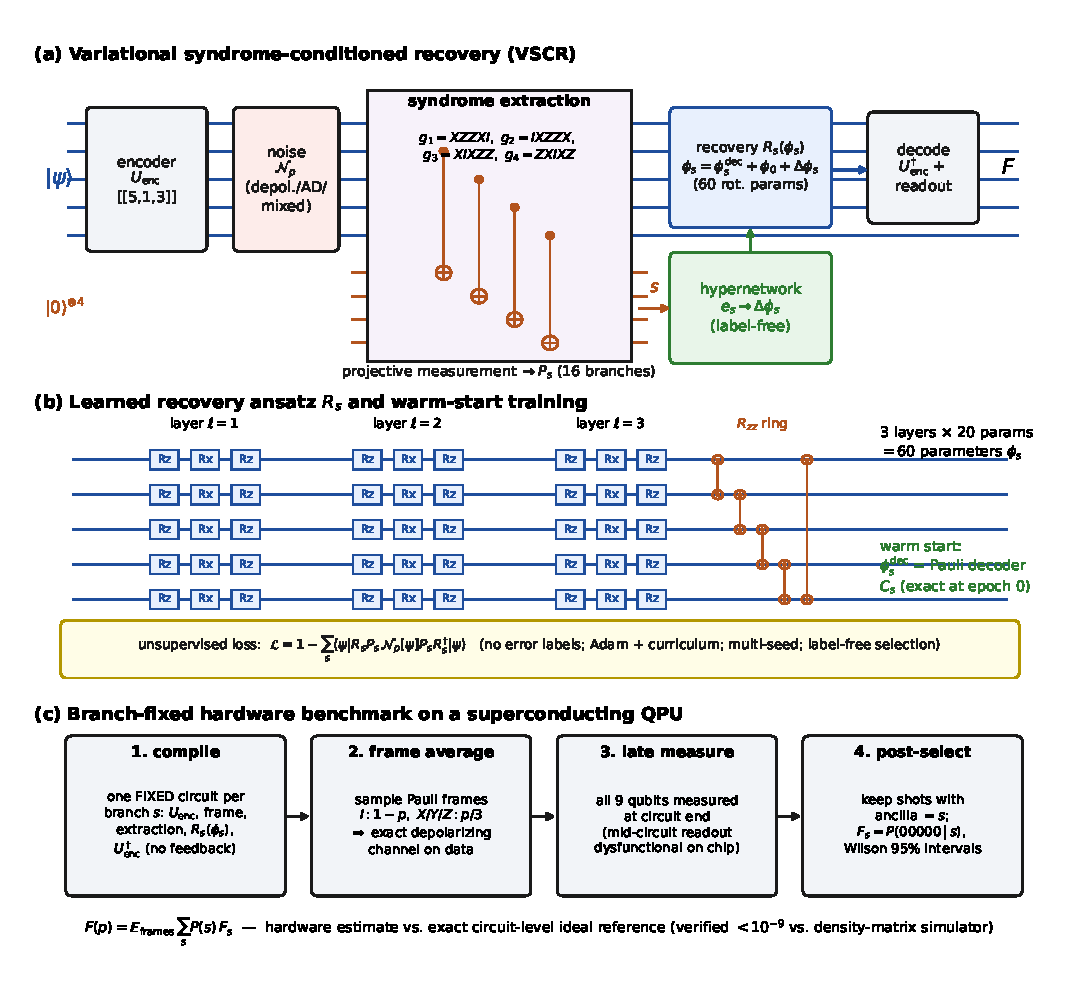
\includegraphics[width=\textwidth]{fig_schematic.pdf}
\caption{\textbf{VSCR method and hardware protocol.} (a) The instrument:
encoding into the $\code$ code, noise, projective stabilizer extraction onto
four ancillae, hypernetwork-conditioned learned recovery $R_s$, decoding and
readout. (b) Recovery ansatz and decoder-warm-start parameterisation.
(c) Branch-fixed hardware benchmark: compilation, exact Pauli-frame
averaging, late measurement, post-selection.}
\label{fig:schematic}
\end{figure}

\begin{figure}[ht]
\centering
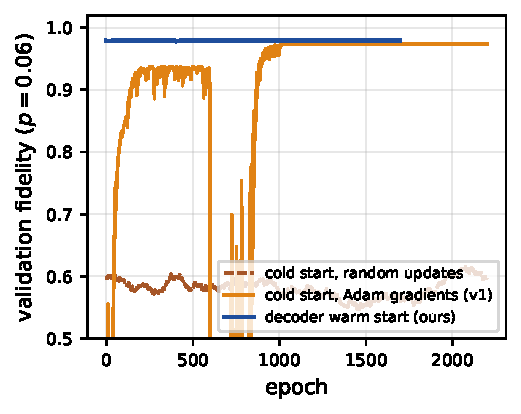
\includegraphics[width=0.55\textwidth]{fig_training.pdf}\\[4pt]
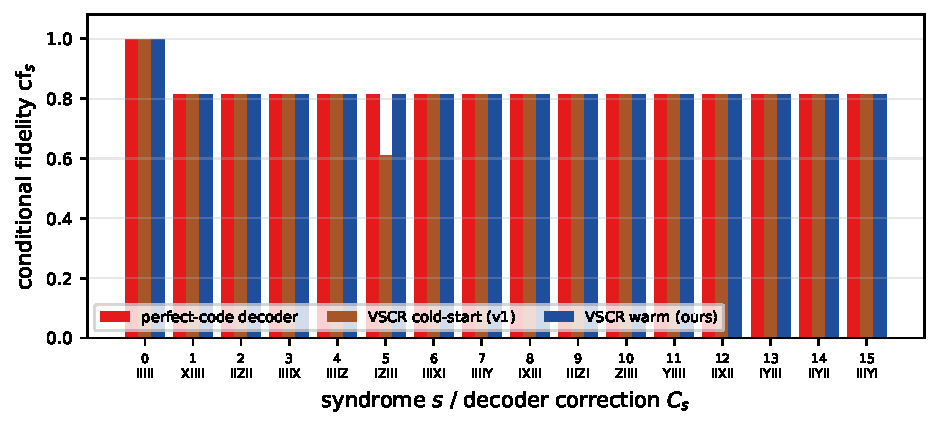
\includegraphics[width=\textwidth]{fig_branch_cf.pdf}
\caption{\textbf{Training and per-branch health.} (a) Validation fidelity for
decoder-warm-started Adam training versus cold-started training and
gradient-free random updates. (b) Per-syndrome conditional fidelity
$\mathrm{cf}_s$ at $p=0.15$ (depolarizing) for the Pauli decoder, the
cold-started model and the warm-started model: the warm start removes the
unhealthy branches of cold-started variational recovery while reaching the
decoder on every branch.}
\label{fig:training}
\end{figure}

\begin{figure}[ht]
\centering
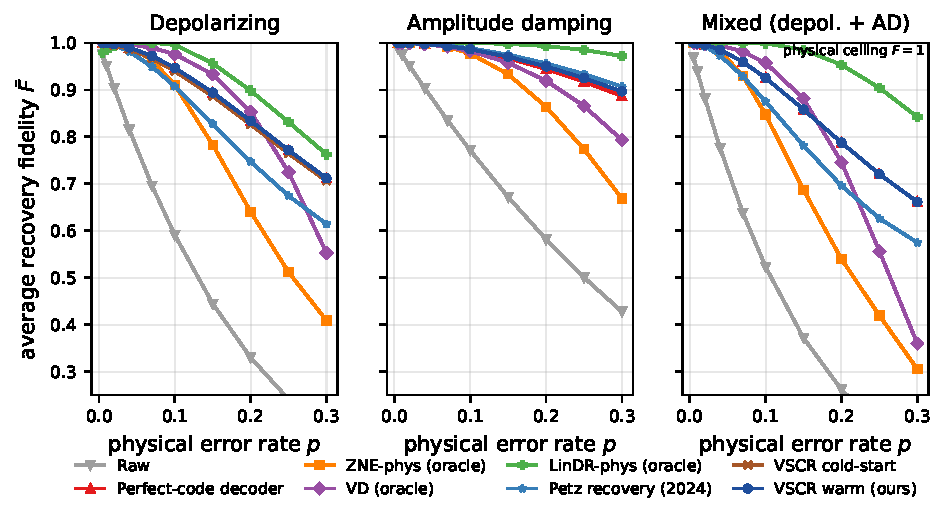
\includegraphics[width=\textwidth]{fig_sim_benchmark.pdf}\\[6pt]
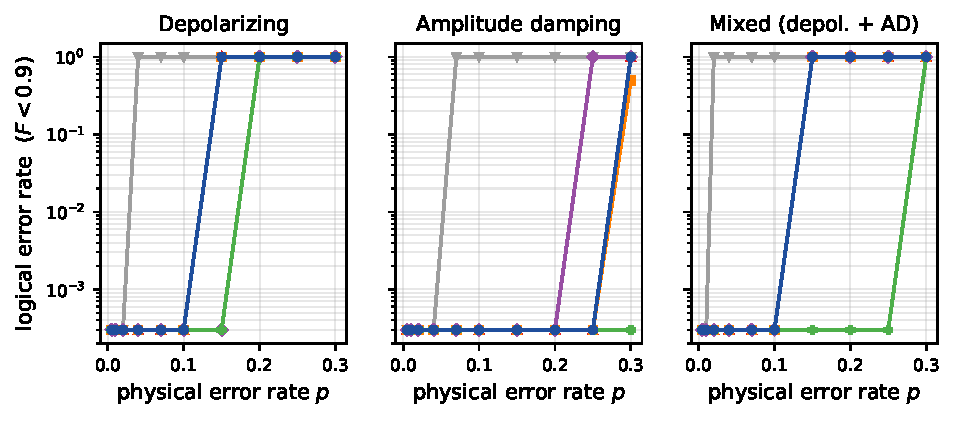
\includegraphics[width=\textwidth]{fig_sim_ler.pdf}\\[6pt]
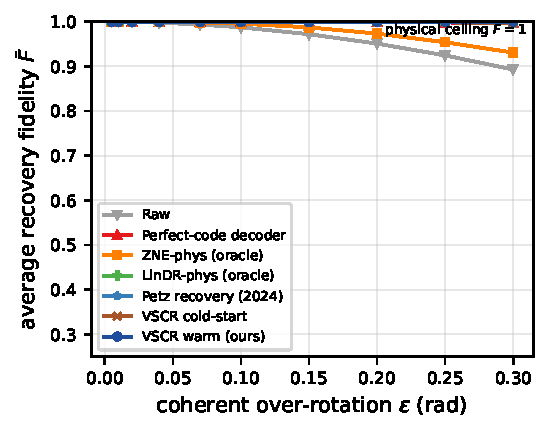
\includegraphics[width=0.62\textwidth]{fig_coherent.pdf}
\caption{\textbf{Recovery benchmarks.} Average fidelity (top) and logical
error rate $\Pr(F<0.9)$ (middle) versus physical error rate for depolarizing,
amplitude-damping and mixed noise; coherent over-rotation channel (bottom).
Bands: standard error over $200$ random logical states. Every method is scored
on a \emph{physical} state, so all fidelity axes are capped at exactly $1$ with
the physical ceiling $\bar F=1$ drawn as a dotted reference line, and the
evaluation asserts $\bar F\le1+10^{-9}$ for every method at every noise
strength. Zero-noise extrapolation is reported \emph{projected} (ZNE-phys): the
raw Richardson estimator is an unbounded linear functional of the extrapolated
operator and exceeds $1$ on the coherent channel for \emph{every} audited state
at \emph{every} strength (up to $1.1306$ at $\varepsilon=0.30$), whereas on the
three incoherent channels it never does ($0/60$ states); an unprojected ZNE curve
would therefore appear to win that panel purely by leaving the physical state
space (Methods). Virtual distillation is omitted from the
coherent panel because $\rho^2=\rho$ there makes it algebraically identical to
Raw; that identity is asserted to machine precision ($1.6\times10^{-15}$) rather
than plotted as a duplicate curve. \emph{Petz recovery (2024)} is the
noise-adapted recovery channel of Eq.~\ref{eq:petz}, scored with the identical
estimator. Warm-started VSCR coincides with the perfect-code decoder on
depolarizing and mixed noise, where the decoder is provably CPTP-optimal
(certified headroom $\le10^{-15}$; ED Table~7), and separates \emph{above} it on
amplitude-damping and coherent noise---at $p=0.10$ amplitude damping
$\bar F=0.98635$ versus $0.98475$ for the decoder, and at $\varepsilon=0.30$
$\bar F=0.99997$ versus $0.99688$---where the separable refinement of Methods
captures $90\%$ and $99.9996\%$ respectively of the certified non-Pauli
headroom. In all cases the decoder floor guarantees
$\bar F_{\rm warm}\ge\bar F^{\rm dec}$ by construction.}
\label{fig:benchmark}
% NB: the coherent over-rotation channel is the BOTTOM PANEL of this same float
% (fig_coherent.pdf above), not a separate figure. It therefore deliberately has
% no `fig:coherent` label of its own: a second label on one float would resolve to
% the same number and read as a dangling self-reference. Point readers at
% Fig.~\ref{fig:benchmark} and say "bottom panel".
\end{figure}

\begin{figure}[ht]
\centering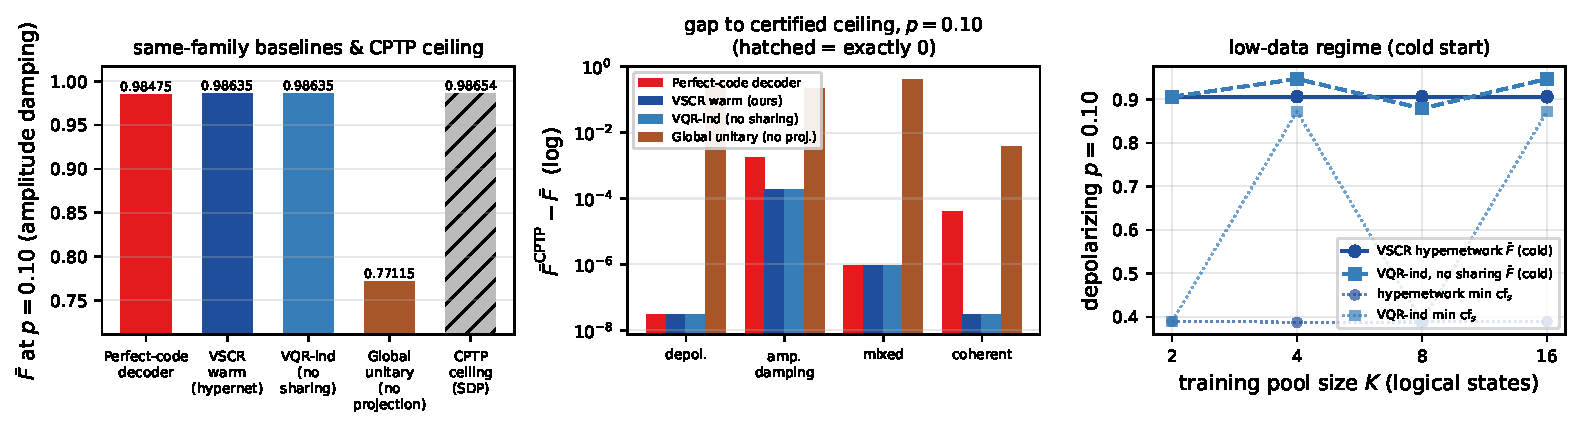
\includegraphics[width=\textwidth]{fig_ablation.pdf}
\caption{\textbf{Same-family baselines, gap to the certified ceiling, and
low-data ablations.} (a) \emph{Amplitude damping} at $p=0.10$: perfect-code
decoder, warm-started VSCR (hypernetwork), VQR-ind (per-syndrome independent
angle table, no sharing), a global variational unitary without syndrome
projection (QVECTOR-style), and the SDP optimal CPTP ceiling (hatched). This
panel was previously the depolarizing comparison, in which the decoder, both
learned architectures and the ceiling agreed to $7\times10^{-12}$ because the
rigid Pauli decoder is \emph{exactly} CPTP-optimal on that channel
($\max_s$ branch gap $=0.0$, ED Table~7). That tie is the statement of a
theorem, not a null result---but a linear-scale bar chart of quantities
differing by $10^{-11}$ has no visual discrimination by construction. Amplitude
damping is the channel on which the bars genuinely separate (the ceiling exceeds
the decoder by $1.8\times10^{-3}$, and the worst single branch by $+0.195$), so
panel (a) uses it; the depolarizing values are still computed and reported so
that the identity remains auditable. (b) \emph{New}: the gap to the certified
CPTP ceiling, $\bar F^{\rm CPTP}-\bar F$, on a log scale for all four channels.
A log gap is the only presentation in which an exact $0$ (depolarizing, where
every syndrome-resolved method sits at the ceiling: hatched and labelled),
$9\times10^{-7}$ (mixed), $1.8\times10^{-3}$ for the decoder against
$1.9\times10^{-4}$ for VSCR (amplitude damping), $4.1\times10^{-5}$ against
$6.8\times10^{-9}$ (coherent---a factor of $6000$, the clearest single view of
what the refinement buys) and $4\times10^{-1}$ (the projection-free global
unitary) are simultaneously legible. The panel spans eight orders of magnitude,
and it turns the depolarizing tie from an uninformative visual coincidence into a
quantitative claim about how close each method is to optimal. (c) Low-data regime:
cold-started training on a fixed pool of $K$ logical states (depolarizing,
evaluated at $p=0.10$ on $200$ fresh states); solid lines: average fidelity
$\bar F$, dotted: worst-branch conditional fidelity $\min_s\mathrm{cf}_s$.}
\label{fig:ablation}
\end{figure}

\begin{figure}[ht]
\centering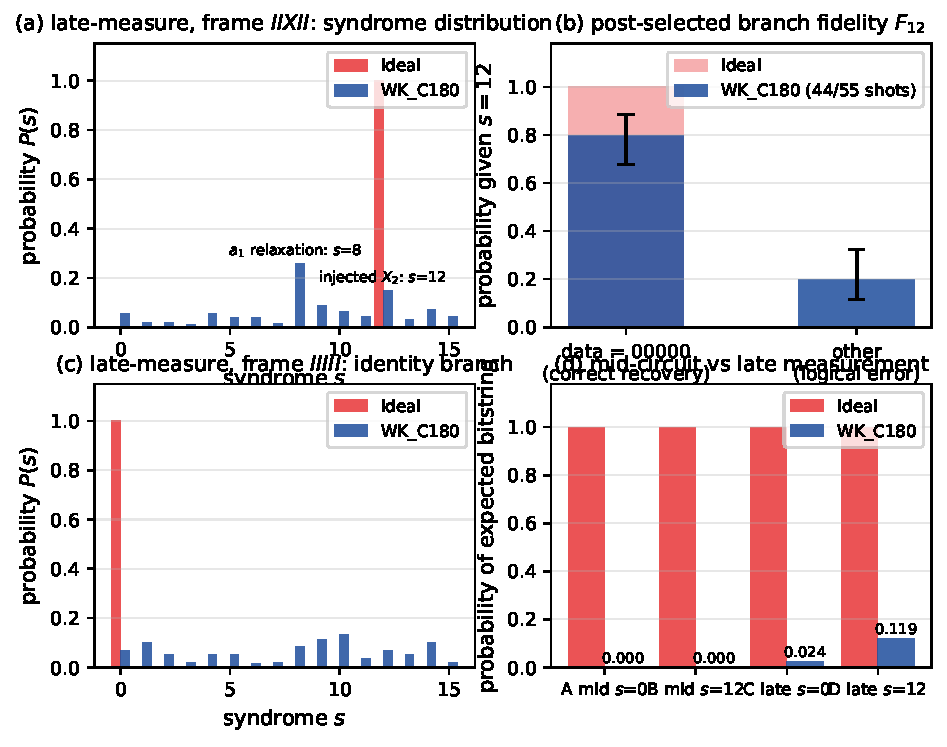
\includegraphics[width=\textwidth]{fig_hw_feasibility.pdf}
\caption{\textbf{Hardware feasibility on OriginQ Wukong \texttt{WK\_C180}.}
(a) Syndrome distribution for the late-measure circuit with injected $X_2$
(frame $IIXII$): hardware peak at $s=12$ with ancilla-relaxation satellite
$s=8$, versus the ideal delta. (b) Post-selected recovery fidelity
$F_{12}=0.80$ ($44/55$ shots, Wilson $95\%$ interval) against ideal $1.0$.
(c) Identity branch: hardware syndrome distribution nearly uniform.
(d) Probability of the expected bitstring per circuit: mid-measure circuits
yield no signal; late-measure circuits retain syndrome correlation.}
\label{fig:hardware}
\end{figure}

\bibliography{refs}
\bibliographystyle{unsrtnat}

\end{document}
